\chapter{SleeveAR}
\label{sec:sleevear}

\section*{Summary}

Before implementing SleeveAR, it was vital to fully establish what were our goals and what we wanted to achieve. 
The following chapter describes our vision of this work and lists the feautures we considered to be a minimum requirement for a successful implementation.



\section{Vision}

\begin{figure*}[!t]
    \begin{center}
        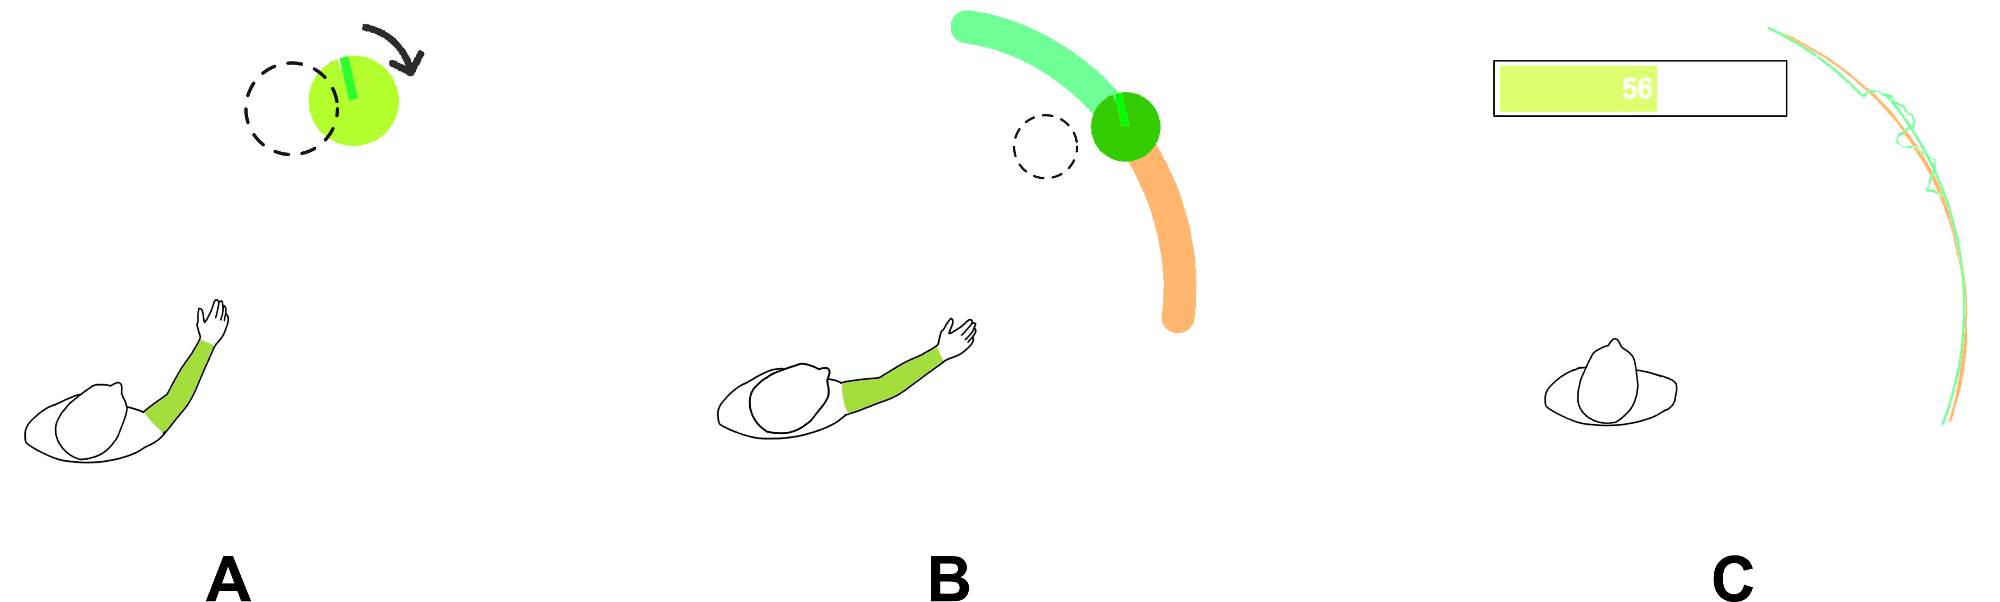
\includegraphics[width=0.9\textwidth]{imgs/interaction.png}
    \end{center}
    \caption{Sleeve Projected Feedback: A) bla. B) Bla. C) Bla}
    \label{fig:interaction}
\end{figure*}

SleeveAR aims further beyond the accomplishments LightGuide was able to make. 
As described in the previous section, Lightguide only focused on projecting information on top of the hand. Not only does this leave a small room for movement variety, but also the amount of possible information given can be quite reduced.
By increasing the projection area throughout the whole arm we can successfully improve an user's awareness while an movement is being executed. 
Not only that, but if it was possible for the movement being replicated to be originated by another person, we could achieve much more realistic and useful guidance.
With SleeveAR virtual content can be projected onto different surfaces, and even, onto people's own limbs, to provide, in real-time, a more immersive experience. 

Our vision consists on two main concepts. Firstly, the precise recording of the exercise being demonstrated by a personal therapist. 
And secondly, the ability to properly guide another person, the rehabilitation subject, during the execution of the pre-recorded exercise. 
While, at the same time, provide awareness of the rehabilitation exercise progress to insure the correctness of the patient's movements.
With SleeveAR, a therapist can easily demonstrate the prescribed exercises and make sure his patient will perform them correctly without the requirement of his close supervision.

In the SleeveAR system, the exercise being performed needs to be recorded beforehand, which, in this case, should be a health professional. 
Not only it provides a great range of possible movements, but also assigns,onto the professional, the responsibility of providing adequate exercises based on a specific patient's condition


\section{Visual Feedback}

To provide feedback that a user would understand naturally, we aimed at a minimalist design that the user could find easy to understand. 
Our main goal was for a user to observe the visual cues being projected and imediatly understand what had to be done to correct his arm.

With this in mind, we divided our visual feedback into two main components. 
First, the \textbf{elbow angle}, given by the relative angle between the upper and fore arm regions \todo{picture of the arm anatomy?}. 
Second, the \textbf{upper arm direction} given by the direction from the shoulder to the elbow.


\subsection{Elbow Angle}

Given the fore arm movement being restricted by the upper arm, its range of movement could be simplified in terms of flexing and extending, therefore, increasing and decreasing the elbow angle as seen on Figure \todo{figura de braço a flectir e extender}.

To provide visual feedback for the elbow angle, it was necessary to present the current angle and the desired angle to be achieved at the same time. So the user could be aware of his current arm pose and visualize to where he should move his forearm to correct it.

\todo{figura do circulo elbow angle}

Figure \todo{figura} shows two examples of our feedback design. The black bar represents the user's current elbow angle. On the other hand, the green bar represents the desired angle that must be achieved. 

\subsection{Upper Arm Direction}


\section{Movement Guidance}
Hereafter, as depicted in Figure~\ref{fig:vision}, 
the patient follows all provided feedback to replicate the pre-recorded movement step-by-step, without ever seeing the exercise executed before.
The current position of the subject's arm is being constantly tracked in order to always provide real-time 
feedback based on how he should move it from that point.
Visual feedback is achieved by projecting light onto his full arm and surroundings. The projection on the arm will enable us to 
guide a subject through translations and rotations, using different kinds of visual cues to different situations. As for the projection on the subject's surrounding 
will serve the purpose of providing other useful information not directly connected to the movement itself. 
In Figure~\ref{fig:vision} we can observe a progress bar being projected on the floor. 
This bar not only provides the subject an understanding of how far in the exercise he is at the moment, but also helps the subject visualize the angle of movement he should be doing.
Audio and haptic feedback can help inform the subject about specific information, without making him loose his focus on the visual feedback.
The haptic feedback is used to quickly notify the subject of any vital information about the current state of the exercise. 
Awareness of erroneous movements is achieved mainly by the employment of vibration cues into the patient's arm.
Furthermore, for the purpose of timing, auditory feedback provide the subject with information regarding when to start or stop the exercise by using recognizable audio cues which represent those same actions.

Interactive phases(Figure~\ref{fig:interaction}):
\begin{itemize}
\item {\bf Initial Position Phase:}
\item {\bf Task Performance:}
\item {\bf Progress Report:}
\end{itemize}



\begin{figure}[!b]
    \begin{center}
        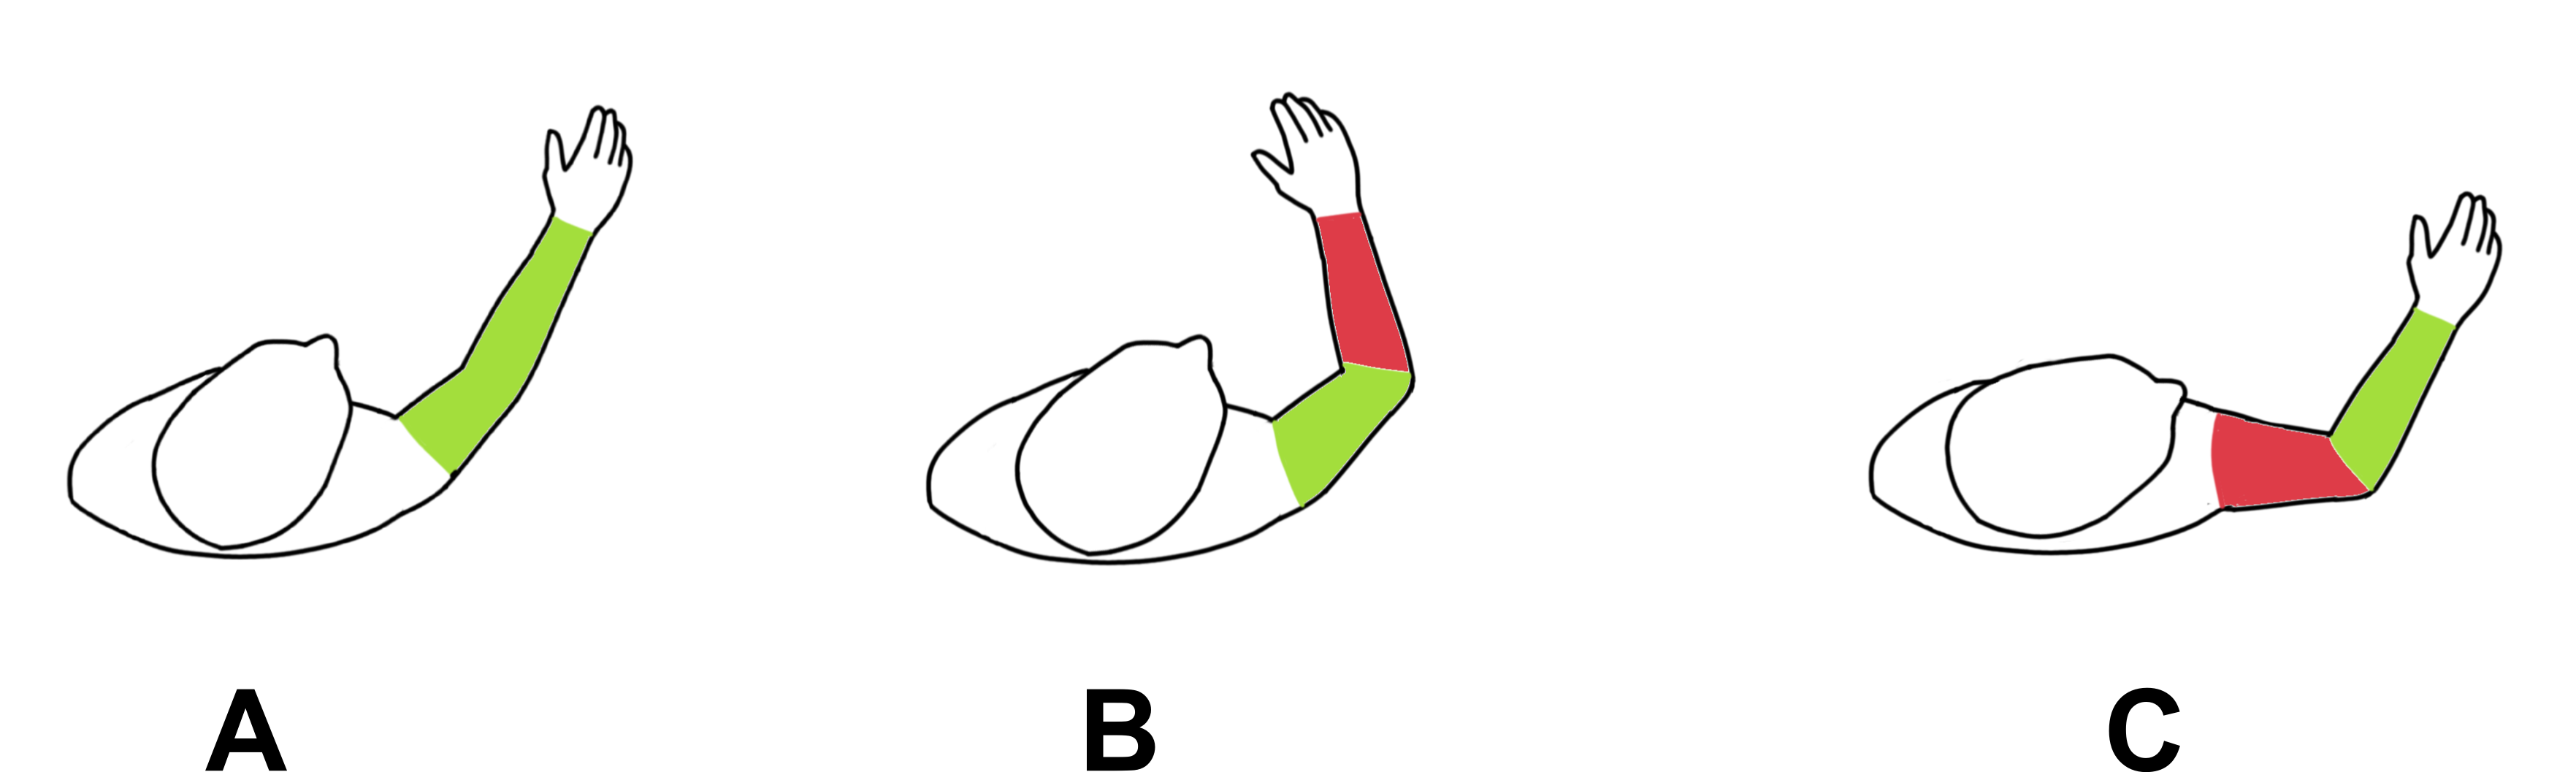
\includegraphics[width=\columnwidth]{imgs/visualfeedback.png}
    \end{center}
    \caption{Sleeve Projected Feedback: A) bla. B) Bla. C) Bla}
    \label{fig:vision}
\end{figure}